% !TeX program = PdfLaTeX
% !TeX root = ../Main.tex

\chapter{Introduction to JPAD}
\label{ch1}

Nowadays the preliminary design phase of an aircraft is becoming very challenging due to the need for more demanding requirements which deals with different fields of applications. In this perspective, there is a certain need for simple design tools both in aircraft industries and academic research groups which can perform fast and reliable multi-disciplinary analyses and optimizations.

This chapter provides a comprehensive overview of JPAD (Java toolchain of Programs for Aircraft Design), a Java-based open-source library conceived as a fast and efficient tool useful as support in the preliminary design phases of an aircraft, and during its optimization process. The library has been completely realized at the Department of Industrial Engineering of the University of Naples “Federico II” where is still in development.

One of the main features of JPAD lies in the smart management of both the aircraft parametric model, which is conceived as a set of interconnected and parameterized components, and the available analyses. The library has been developed with the purpose of simplify the composition of the input file for the user and doing fast analysis with a satisfying grade of accuracy. The following section will focus on the description of the software structure and its main advantages. Another key point is the possibility to easily interface JPAD with other external tools in order to achieve a higher level of accuracy.

The JPAD library is an alternative to a plethora of similar software tools, both freeware and commercial. Most of these tools have an important history, and many of them have been in use for decades. Some of them were conceived with poor software design criteria, have a rigid textual input and come with no visualization features. This is the main reason why JPAD has been developed paying a lot of attention to simplicity and flexibility. Moreover, it has been conceived as an open-source tool.

% --------------------------------------------------------------------------------------------------------------------------------------------
% SEZIONE 1
% --------------------------------------------------------------------------------------------------------------------------------------------
\section{Software structure}
\label{sec1.1}

To achieve a clear input file organization a considerable study has been done. The result is an input structure composed by different XML files with the purpose to allow users to easily manage all data needed to execute the desired analyses. In figure~\vref{JPADSchematicFlowChart} the entire structure of the software is schematized. It is possible to clearly note that there are two main blocks: input and core.

\begin{figure}[htbp] 
\centering
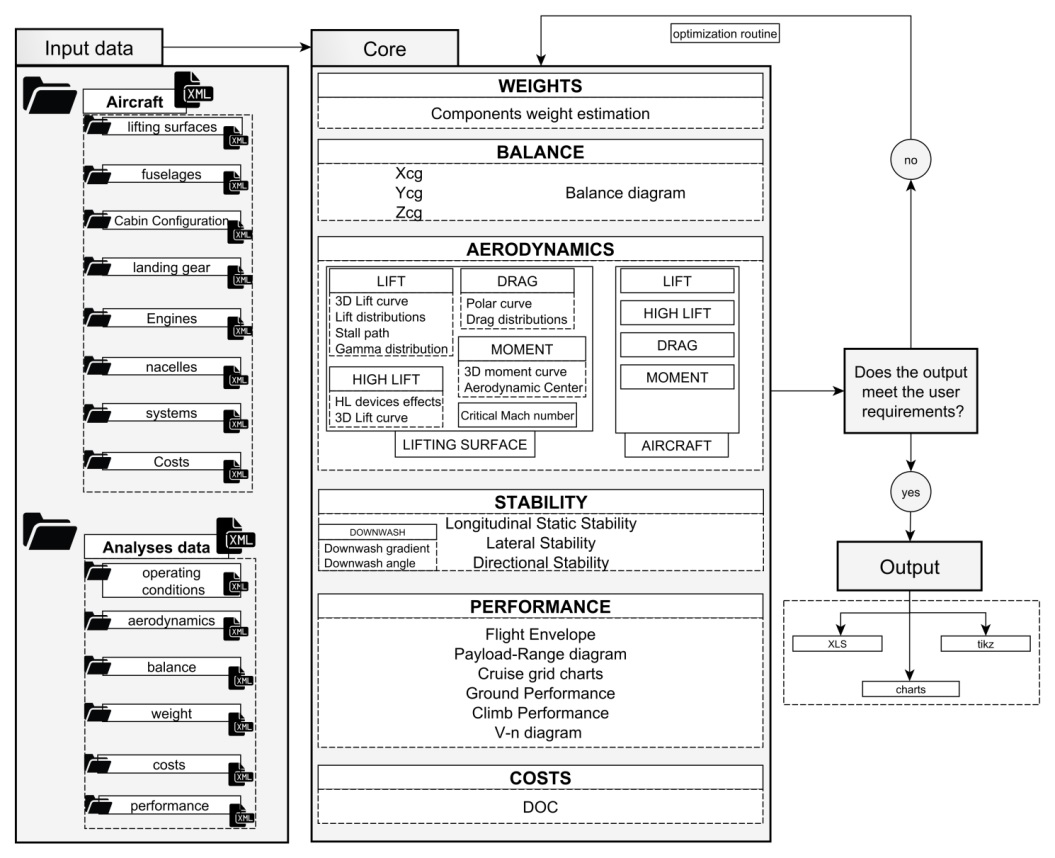
\includegraphics[height=0.45\textheight]{Immagini/Capitolo1/1_1-JPADSchematicFlowChart}
\caption[JPAD schematic flow-chart] {JPAD schematic flow-chart}
\label{JPADSchematicFlowChart}
\end{figure}

\begin{figure}[htbp] 
\centering
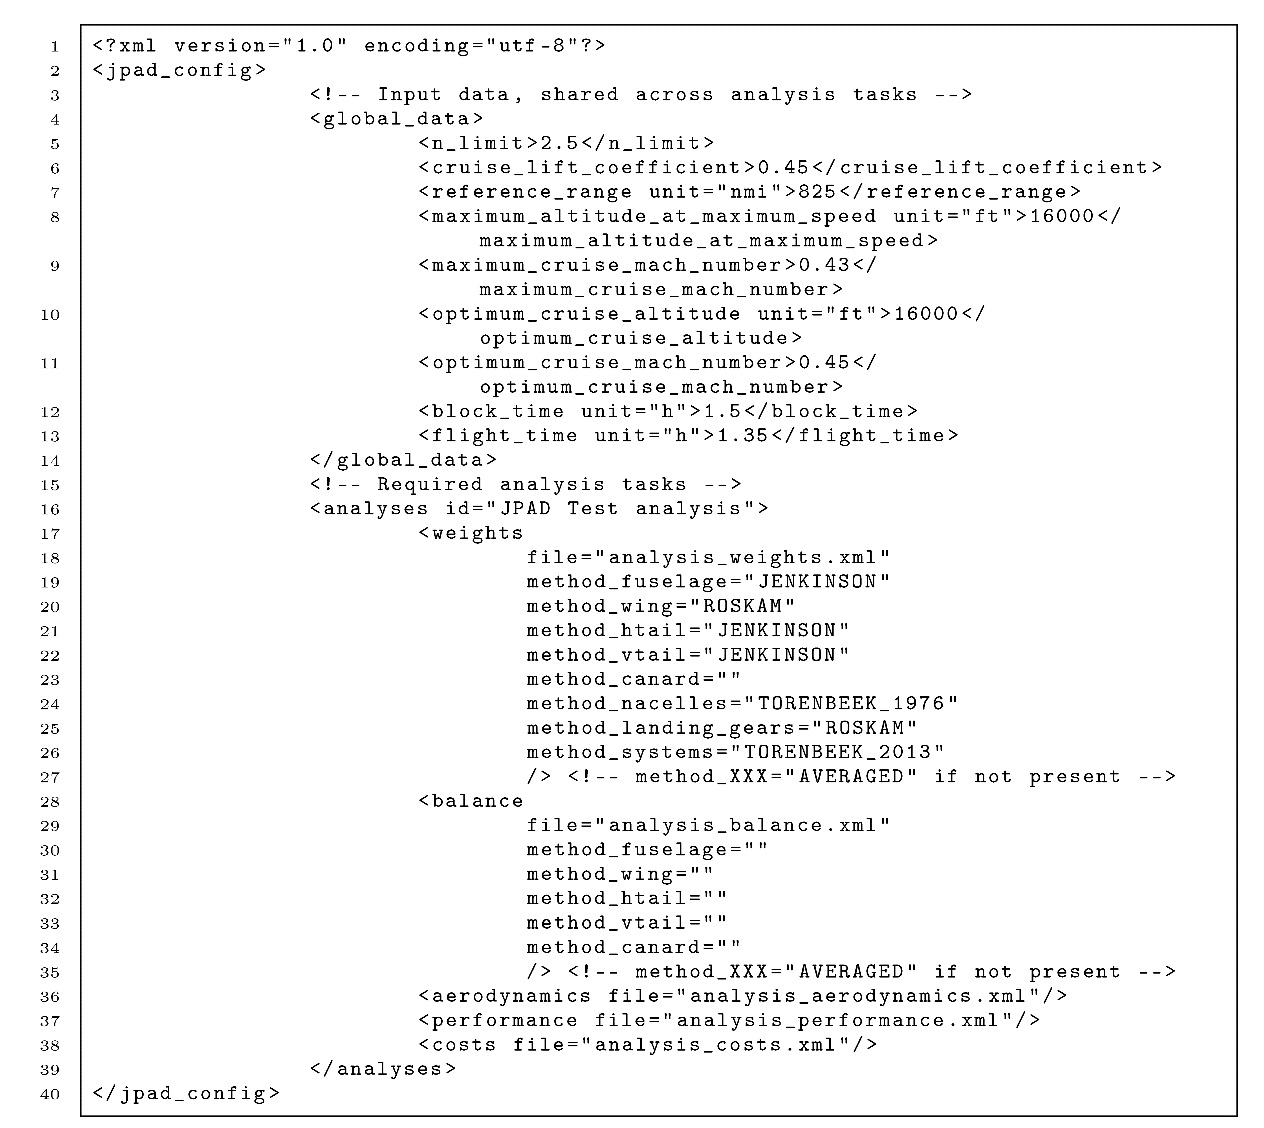
\includegraphics[height=0.45\textheight]{Immagini/Capitolo1/1_2-AnExampleOfTheAnalysisXmlFile}
\caption[Example of analysis.xml file] {An example of the analysis.xml file}
\label{AnExampleOfTheAnalysisXmlFile}
\end{figure}

\begin{figure}[htbp] 
\centering
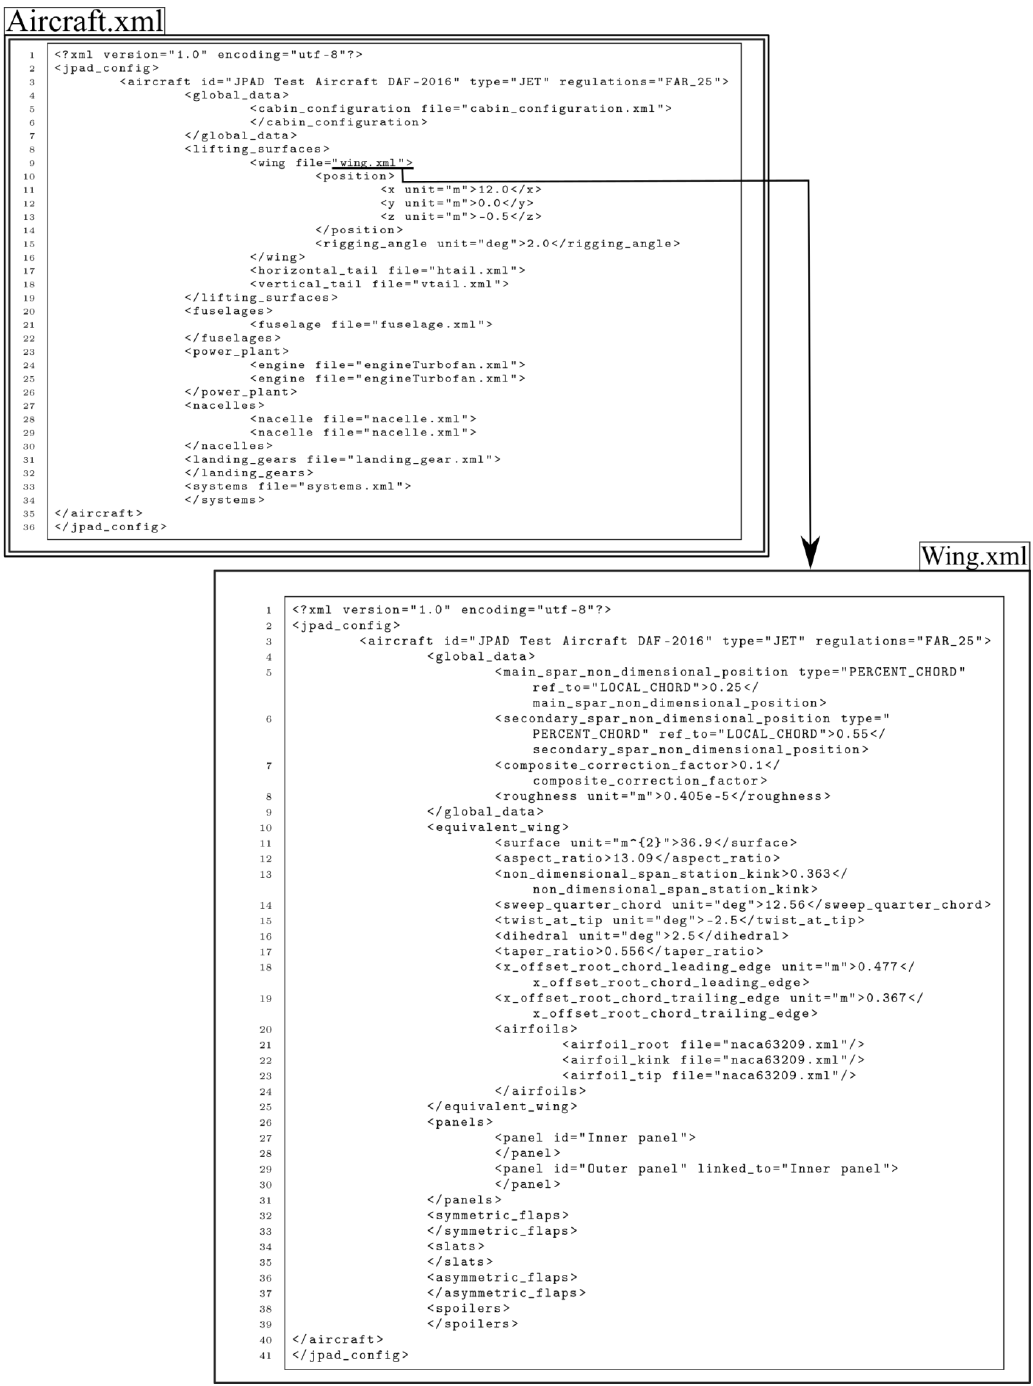
\includegraphics[width=\textwidth]{Immagini/Capitolo1/1_3-AnExtractFromAGeneralAircraftXmlInputFile}
\caption[Extract from general Aircraft.xml input file] {An extract from a general Aircraft.xml input file}
\label{AnExtractFromAGeneralAircraftXmlInputFile}
\end{figure}

The input block is defined by two main parts: aircraft and analyses definitions. The first one defines the aircraft model in parametric way using a main file (Aircraft.xml, see figure~\ref{AnExtractFromAGeneralAircraftXmlInputFile}) which collects all the components, linking them to their related XML file (i.e. fuselage.xml, vtail.xml, and so on) which contains all geometrical data.

The second one defines all necessary data for each analysis presents into core module (see figure~\ref{AnExampleOfTheAnalysisXmlFile}). Since the aircraft model contains only geometrical data, it is necessary to define several further data referred to each analysis. \\

The structure described above allows to generate different aircrafts, or different configurations of the same model, combining different components. The possibility to generate a series of different aircrafts in a simple and fast way, allows to easily perform comparisons between these latter. For example, assuming different wings and engines, it is possible to estimate the effects that some design parameters have on a specific output. Figure~\vref{FAR-25} shows how the FAR-25 take-off field length behaves with different values of the wing surface and the engine static thrust at fixed aircraft maximum take-off weight. This feature plays also a key role in the optimization process described in figure~\ref{JPADSchematicFlowChart}.

\begin{figure}[htbp] 
\centering
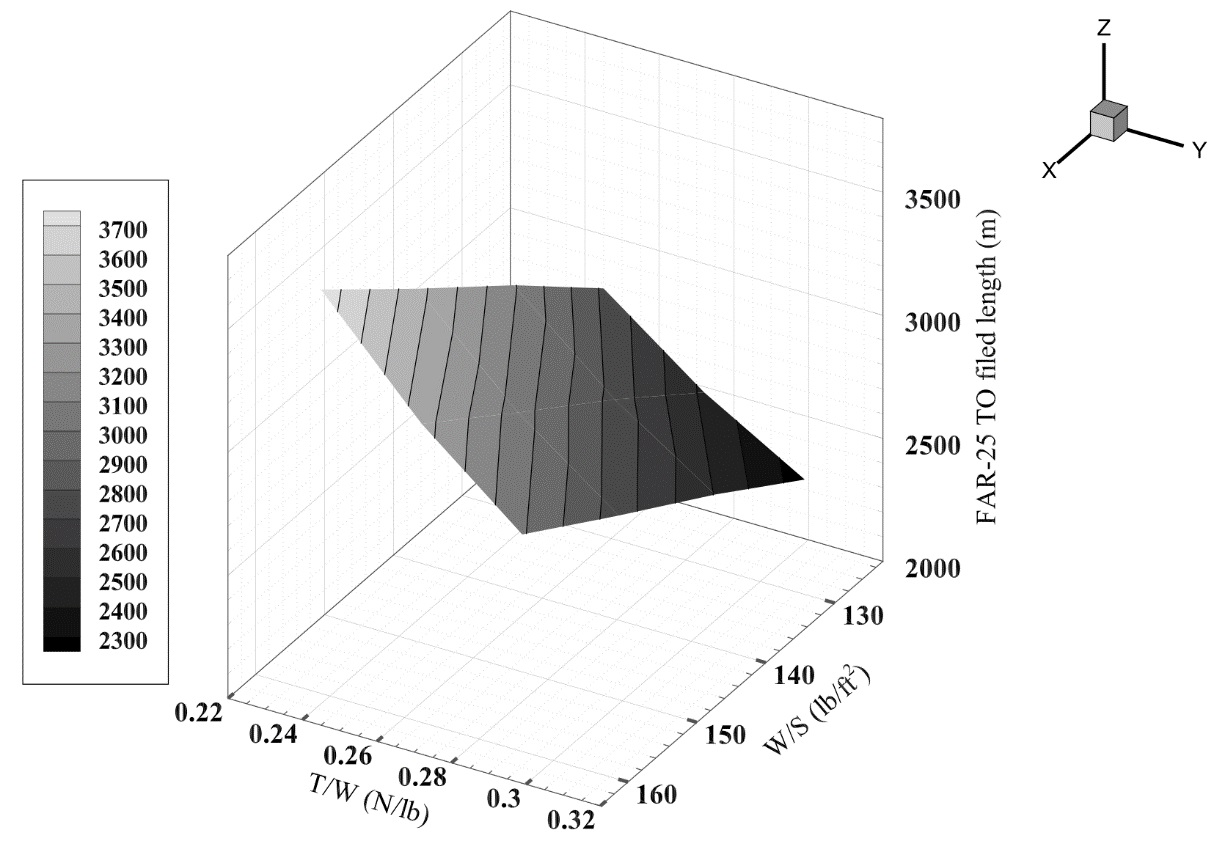
\includegraphics[width=\textwidth]{Immagini/Capitolo1/1_4-FAR-25TakeOffFieldLengthAtDifferentWingLoadingsAndThrustWeightRatios}
\caption[FAR-25 take-off field length at different $W/S_\text W$ and $T/W$] {FAR-25 take-off field length at different wing loadings and thrust-weight ratios}
\label{FAR-25}
\end{figure}

In the same way, it is possible to perform a complete analysis (those present into core block in figure~\ref{JPADSchematicFlowChart}), or a specific one, combining different analyses files. This allows an easier evaluation of generic cost function during optimization tasks, resulting in reduced amount of computational costs required for this kind of operations.

Besides the input, the second main block is the core, which manages all the available analyses. This contains several independent modules, as shown in the figure~\ref{JPADSchematicFlowChart}, that deals with following application fields.
\begin{itemize}
\item Weights: estimates the aircraft weight breakdown starting from a first guess maximum take-off weight and some mission requirements. In particular, it evaluates each aircraft component mass using well-known semi-empirical equations.
\item Balance: estimates the centre of gravity position related to each weight condition and draws the balance diagram.
\item Aerodynamics and Stability: the aerodynamics module estimates all the aerodynamic characteristics concerning lift, drag and moments coefficients at different operating conditions for each aircraft component (wing, tails, fuselage and nacelles), whereas the stability module gives useful data about static stability of the whole aircraft.
\item Performance: evaluates most important aircraft performance such as Payload-Range diagram, mission profile, cruise flight envelope, ground performance, climb performance and the cruise grid chart.
\item Costs: estimates the DOC (Direct Operating Costs) breakdown.
\end{itemize}

Finally, JPAD allows to obtain different kind of output: charts and data in XLS format.

% --------------------------------------------------------------------------------------------------------------------------------------------
% SEZIONE 2
% --------------------------------------------------------------------------------------------------------------------------------------------
\section{The Java Language}
\label{sec1.2}

Java was developed by Sun Microsystems, a company that was incorporated in Oracle from a few years. This programming language is a general-purpose, concurrent, class-based, object-oriented language. It is designed to be simple enough that many programmers can achieve fluency in the language \cite{javaoracle}.

One design goal of Java is portability, which means that programs written for the Java platform must run similarly on any combination of hardware and operating system with adequate runtime support. This is achieved by compiling the Java language code to an intermediate representation called Java bytecode, instead of directly to architecture-specific machine code. Java bytecode instructions are analogous to machine code, but they are intended to be executed by a virtual machine (VM) written specifically for the host hardware. End users commonly use a Java Runtime Environment (JRE) installed on their own machine for standalone Java applications, or in a web browser for Java applets \cite{wiki:java}. \\

There were five primary goals in the creation of the Java language \cite{java}:
\begin{itemize}
\item it must be ``simple, object-oriented, and familiar'';
\item it must be ``robust and secure'';
\item it must be ``architecture-neutral and portable'';
\item it must execute with ``high performance'';
\item it must be ``interpreted, threaded, and dynamic''.
\end{itemize}

Actually Java is the most used programming language according to TIOBE (see figure~\vref{TIOBE}). The TIOBE Programming Community index is an indicator of the popularity of programming languages. The ratings are based on the number of skilled engineers world-wide, courses and third party vendors.

\begin{figure}[htbp]
\centering
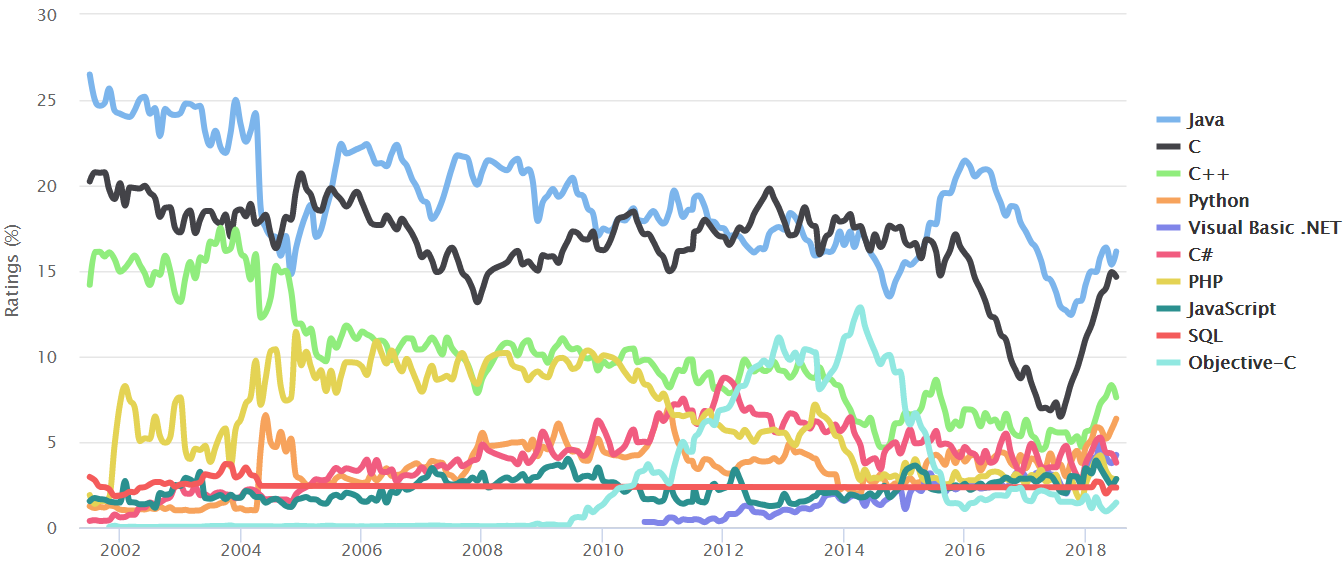
\includegraphics[width=\textwidth]{Immagini/Capitolo1/1_5-TrendTIOBE} 
\caption{TIOBE Programming Community index (\href{www.tiobe.com}{www.tiobe.com})}
\label{TIOBE}
\end{figure}

% --------------------------------------------------------------------------------------------------------------------------------------------
% SEZIONE 3
% --------------------------------------------------------------------------------------------------------------------------------------------
\section{Java choice}
\label{sec1.3}

The choice of Java as the programming language was driven by several considerations. These include the following:
\begin{itemize}
\item the language should be widely supported; this to avoid the case of many valid aircraft design applications and libraries that became obsolete due to the aging of the programming language used to build them;
\item the language is object oriented;
\item the language should promote the use of open source libraries, especially for I/O tasks and for complex mathematical operations;
\item the language and the companion Integrated Development Environment (IDE) should provide a widely supported Graphical User Interface (GUI) framework and a GUI visual builder;
\item the language should support and promote modularity.
\end{itemize}

The Java programming language meets all these requirements; moreover it is backed by Oracle and by a huge community of developers so it is continuously updated. Also, advanced and free IDEs (such as Eclipse) allow programmers to streamline and simplify the development process; in particular, the Eclipse IDE has been chosen to develop JPAD.

Being Java a pure object oriented programming language, it greatly encourages and simplifies modularization. Each module (package) can be programmed quite independently so that it is relatively easy to divide the work among several programmers. This is essential since the amount of classes and calculations needed to abstract, manage and analyse the entire aircraft is very large (presently the whole project counts more than 10 millions lines of code). For such a reason the establishment of common practices and the adherence to fundamental principle of software development (\emph{Don’t Repeat Yourself}, \emph{Separation of Concerns}, \emph{Agile software development}) are equally important.